\chapter{Linear Collider Concepts}
\section{Beam line description}
% \section{Optics}
\subsection{Beam Delivery System (BDS)}
After the acceleration, in the Beam Delivery System (BDS) the beam needs to be focused and higher order aberrations must be compensated to obtain nanometer beam size. 
\subsection{Final Focus Sections (FFS)}
In the Final Focus Section (FFS) the goal is to minimize the beam size. If the lattice is conceived as a telescope where the matrix elements are as in Eq.~(\ref{eq:telescope}), being $M_x, M_y$ the magnifications in horizontal and vertical planes, then, beam size to the first order does not depends on the energy spread $\delta$. Considering the second and third order components in the transfer map, as in Eq.~(\ref{eq:tmap}), then, the telescope properties show that the main contribution to beam size is chromaticity $\xi_{x\atop y}$ given by the elements $T_{126},$ and $T_{346}$~\cite{Brown:1987}, identified in~\cite{GarciaMorales:1982827} as
\begin{equation}
 \xi_x = \frac{1}{\beta_x^*}\left(T_{116}^2\beta_{x0}+T_{126}^2\frac{1}{\beta_{x0}}\right)\qquad
 \xi_y = \frac{1}{\beta_y^*}\left(T_{336}^2\beta_{y0}+T_{346}^2\frac{1}{\beta_{y0}}\right)
\end{equation}
being the 0-index the values at the input and *-index the values at the output. For this reason, the FFS has been conceived as a telescope to demagnify the beam size with minimum effect of energy spread, where the main issue is the large chromaticity generated at the Final Doublet (FD), the last pair of quadrupoles which focus the beam at the Interaction Point (IP).
\begin{equation}
R=
 \begin{pmatrix}
   M_x & 0 & 0 & 0 \\
   0 & 1/M_x & 0 & 0 \\
   0 & 0 & M_y & 0 \\
   0 & 0 & 0 & 1/M_y \\
  \end{pmatrix}\label{eq:telescope}
\end{equation}
\begin{equation}
x_i=\sum_{j=1}^6R_{ij}x_j+\sum_{j,k=1}^6T_{ijk}x_jx_k+\sum_{j,k,l=1}^6U_{ijkl}x_jx_kx_l+\cdots\qquad x_i\in x,x',y,y',\tau,\delta\label{eq:tmap}
\end{equation}
\section{Overview of FFS effects}
\subsection{Chromaticity}
As in the case of light beams through lenses, the longitudinal focal point location depends on the beam energy spread. This effect is called chromaticity.  Figure~\ref{f:chrom} represents schematically the focusing effect of a magnet as a lens. A particle with the design momentum crossing the lens at a distance $y_0$ from the center will be focused at $l^*$. Off-momentum particles with higher or lower momentum will be under-focused or over-focused, respectively. This produces a variation in the transverse position at the focal distance $l^*$ increasing the beam size.\par
\begin{figure}[!hbt]
\centering
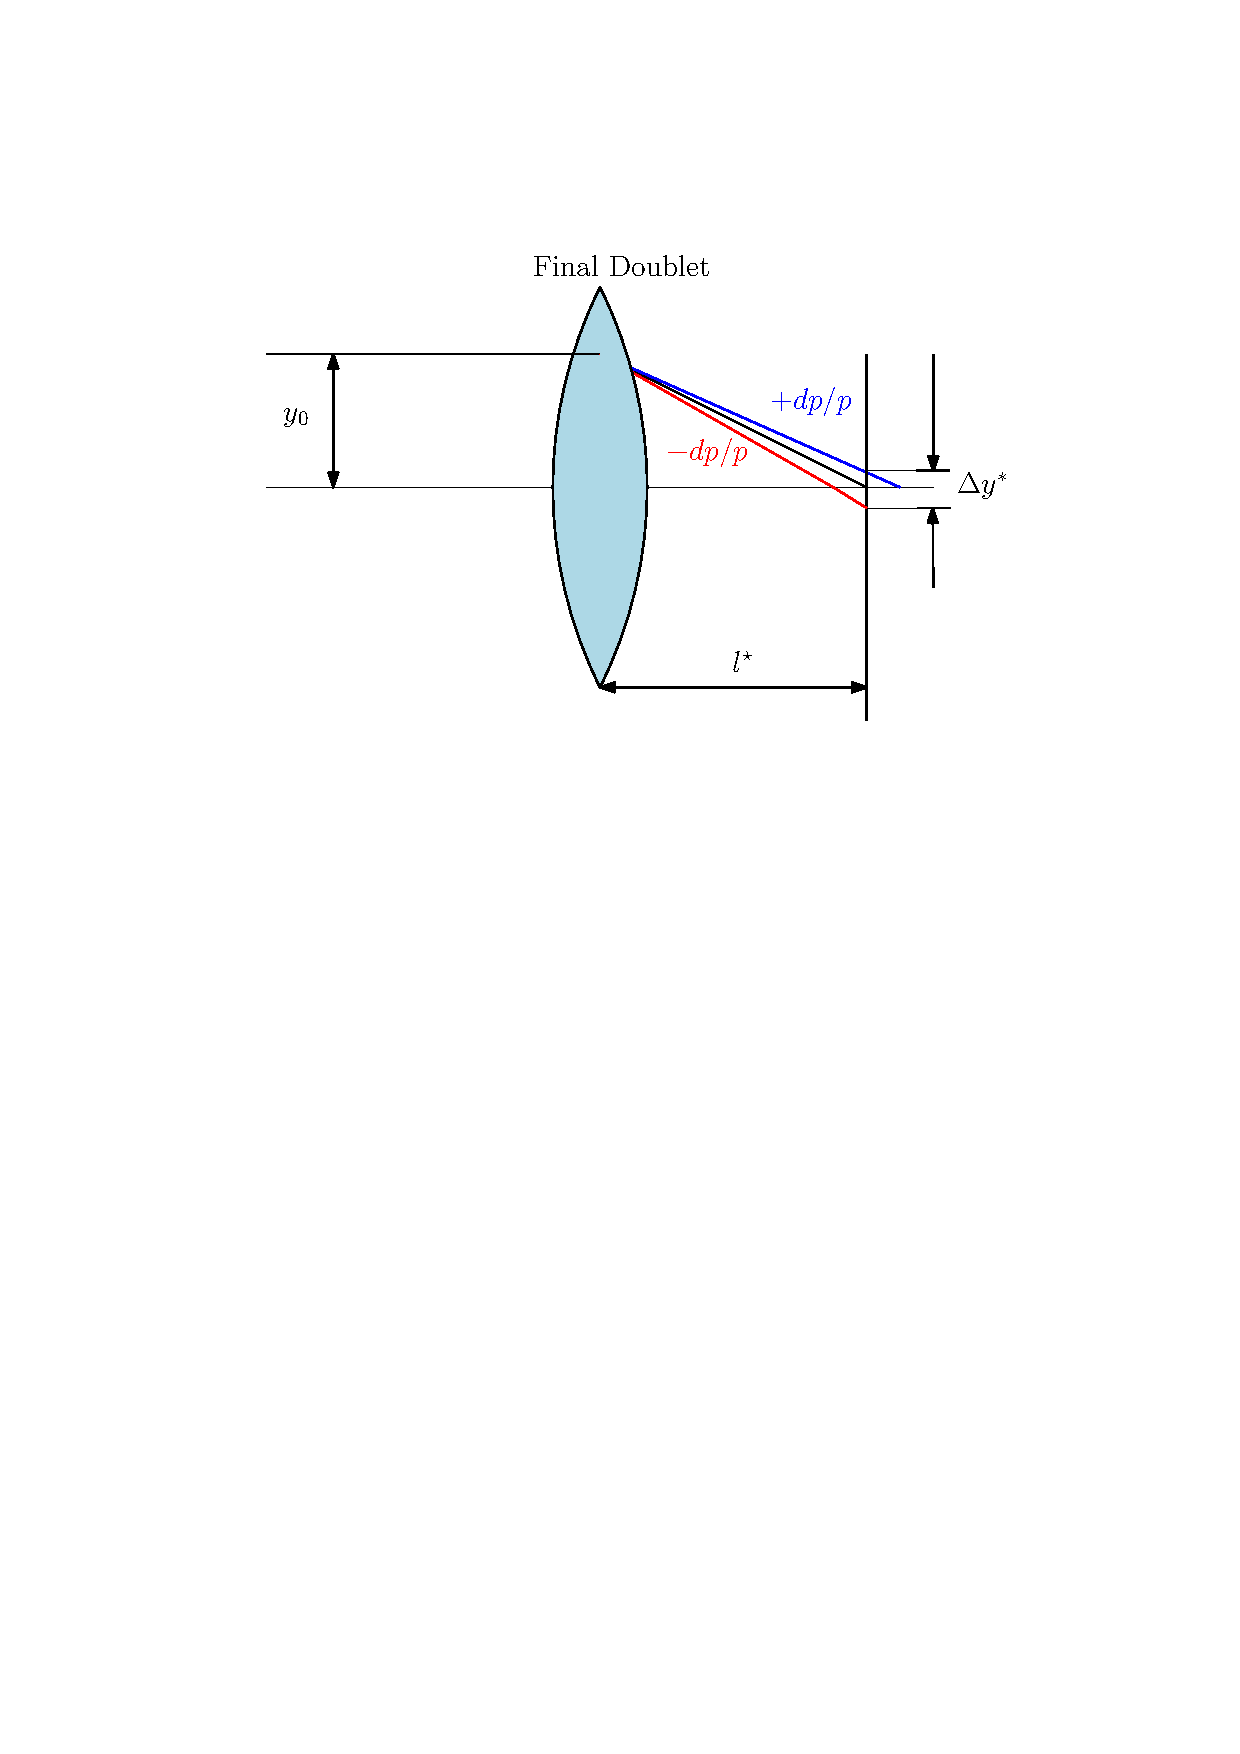
\includegraphics[scale=0.5]{chromaticity.pdf}\caption{Chromaticity. Particles with off-momentum energy are focused at different longitudinal locations increasing the beam size.}\label{f:chrom}
\end{figure}
The effect on the beam size is commonly estimated as
\begin{equation}
 \frac{\Delta y^*_{rms}}{\sigma^*_y}\approx\frac{l^*}{\beta^*}\sigma_\delta\approx\xi_y\sigma_\delta
\end{equation}
where $l^*$ is the focal length, $\sigma_\delta$ is the second moment of the energy spread distribution, $\beta_y^*$ is the optical $\beta$ function at the focal position and $\xi_y$ is the chromaticity.\par
The chromatic dilution of the beam size can be expressed as 
\begin{equation}
 \sigma^*_y\approx\sigma_{y,0}\sqrt{1+\xi_y^2\sigma^2_\delta}
\end{equation}
where $\sigma_{y,0}$ is the transverse beam size with zero energy spread.\par
\subsubsection{Chromaticity correction}\label{s:chromcorr}
In the thin lens approximation with a vertically focusing quadrupole magnet of thickness $ds$, the kick in angle given to a crossing particle is expressed in \cite{CAS9104} as
\begin{equation}
 dx'=k_q(1-\delta)xds\qquad dy'=-k_q(1-\delta)yds
\end{equation}
where $dx', dy'$ are the horizontal and vertical angle kick respectively, $k_q$ is the quadrupole gradient and $\delta=dP/P_0$ is the energy spread. A combination of bending magnets and sextupoles is used to substract the extra kick due to energy spread.\par
First, horizontal position and energy are correlated by dispersion, $\eta_x$, generated by bending magnets \cite{CAS9104}. This divides the particle motion in two parts: the betatron motion and an offset equal to $\eta_x\delta$. Equation~(\ref{eq:coortrans}) shows the coordinate transformation.
\begin{align}
 x\rightarrow& x_\beta + \eta_x \delta\label{eq:coortrans}\\
 y\rightarrow& y_\beta\notag
\end{align}
Then, sextupoles are located in dispersive regions ($\eta_x\neq0$) to kick the particles cancelling the quadrupole angle kick dependence on $\delta$. The quadrupole and sextupoles kicks in dispersive region are in Eq.~(\ref{eq:sextkick}), where $k_s$ is sextupole gradient.
\begin{align}
 \text{Quadrupole:}&\qquad dx'=k_q(1-\delta)(x_\beta+\eta_x\delta)ds\qquad& dy'=&-k_q(1-\delta)y_\beta ds \label{eq:sextkick}\\
 \text{Sextupole:}&\qquad dx'=\frac{1}{2}k_s[(x_\beta+\eta_x\delta)^2+y_\beta^2]ds\qquad& dy'=&-k_s(x_\beta+\eta\delta)y_\beta ds\notag
\end{align}
The chromatic terms, $k_q x_\beta\delta$ and $k_q y_\beta\delta$, are cancelled by matching $k_q$ and $k_s\eta_x$.\par
The geometric terms introduced by the sextupole, $\frac{1}{2}~k_s(x^2_\beta+y^2_\beta)$ and $k_sx_\beta y_\beta$, are cancelled by another sextupole, both separated by a transport matrix equal to $-I$ transformation, being $I$ the identity transport matrix.\par
The remaining terms are cancelled by a combination of bending magnets and sextupoles location and strengths. Two methods have been develop to achieve the cancellation all second order terms: the non-local correction and the local correction.\par
%
\textbf{Non-local correction:}~The non-local correction scheme~\cite{Brown:1988} compensates upstream the chromaticity in the FD. Figure~\ref{f-Non-local} shows schematically the lattice configuration, where QF1 and QD0 constitute the FD, B0 to B5 are dipole magnets to produce horizontal dispersion, SD and SF sextupoles are used to cancel vertical and horizontal chromaticity respectively.\par
The chromatic terms, $k_q x_\beta\delta$ and $k_q y_\beta\delta$, are cancelled by making $k_q=k_s\eta_x$.\par
The term $k_q\eta_x\delta$ disappears because the final doublet is in a non-dispersive region.\par
The second order dispersion generated by the sextupoles, $\frac{1}{2}k_s\eta_x\delta^2$, is cancelled by matching the dispersion and sextupole strengths in the $-I$ transformation.
\begin{figure}[h]
   \centering
   \includegraphics*[scale=0.2,angle=0]{nonlocalcorr2.pdf}
   \caption{Non-local chromaticity correction.}
   \label{f-Non-local}
\end{figure}\par
\textbf{Local correction:}~The local chromaticity correction scheme~\cite{Raimondi:2000} compensates chromaticity inside the FD and Fig.~\ref{f-local} shows the sextupoles locations.\par
The non-zero dispersion in the FD generates an offset on the quadrupole horizontal focusing center, $x=x_\beta+\eta_x\delta$.\par
The second order dispersion, $k_q\eta_x\delta^2$ and $\frac{1}{2}k_s\eta_x\delta^2$, is half cancelled if $k_q=k_s\eta_x$. One solution is to double the sextupole strength and produce the entire chromaticity upstream in a non-dispersive region.\par
\begin{figure}[!htb]
   \centering
   \includegraphics[scale=0.2,angle=0]{localcorr2.pdf}
   \caption{Local chromaticity correction.}
   \label{f-local}
\end{figure}
\subsection{Beamstrahlung}
\subsection{Hourglass effect}
Since the $\beta$-functions have their minimum at the IP and increase with the longitudinal distance, to consider the beam size constant along the whole collision length is some cases is not a good approximation. In a low-$\beta$ region 
\subsection{Crossing angle}
\subsection{Tuning}
When considering imperfections, the machine performance decreases dramatically, typically, the beam size increases and luminosity drops substantially about 6 orders of magnitud. The tuning is the procedure which brings the system performance to its design values. Since the initial errors are unknown, the tuning requires a statistical study. Usually more than 100 machines with randomly distributed errors are considered in computer simulations. The simulated tuning reproduces a realistic tuning procedure in a machine \cite{GarciaMorales:1982827,Minty:629879}.\par
